%%
% Please see https://bitbucket.org/rivanvx/beamer/wiki/Home for obtaining beamer.
%%
\documentclass[xcolor=dvipsnames]{beamer} 
\usepackage{graphicx}
\usetheme{Frankfurt}
\setbeamertemplate{items}[circle]
\setbeamertemplate{bibliography item}[text]

% Auto creates the dots for each slide in a section
\usepackage{remreset}
\makeatletter
\@removefromreset{subsection}{section}
\makeatother
\setcounter{subsection}{1}
%\usepackage{dsfont}
%\usepackage{amsmath}
%\usepackage{amssymb}
%\usepackage{amsfonts} 
%\usepackage{mathtools}
%\usepackage{graphicx}
%\usepackage{bm}
%\usepackage{subcaption}
%\usepackage{fancyvrb}
%\usepackage{subfigure}
%\usepackage{graphicx,xcolor}
%\usepackage{pifont,mdframed}
%\usepackage{tikz}
%\usepackage{bm}
%\usetikzlibrary{fit,positioning}




\author{Bryan Feeney} 
\title[Sick Leave Prediction]{A Model to Predict When Employees will take Sick-Leave}
\institute[Mudano]{
 Mudano Interview Process
}
\date[November 17, 2017]{November 17, 2017}

\begin{document}

%--- the titlepage frame -------------------------%


\begin{frame}[plain]
  \titlepage
\end{frame}




%--- Research - MTL -------------------------%


\section{Introduction}
\begin{frame}{Introduction}

Task: Predict when team-members are likely to take sick-leave

\only<2> {
    \begin{itemize}
        \item Sick-Leave Patterns and Indicators
        \item Proposed Model
        \item Evaluation
        \item Engineering
    \end{itemize}
}


\end{frame}

%--- Background ----------------------------------%

\section{Indicators}

\begin{frame}{Sick-Leave Patterns \& Indicators}

\only<1-6> {
    \emph{Sickness absence from work in the UK}\cite{BarhamBegum2005}
}
\only<7> {
\emph{Risk of future sickness absence in frequent and long-term absentees}\cite{Koopmans2008}
}
\only<8> {
\emph{Trends and seasonality in absenteeism}\cite{Akyeampong2007}
}


\only<1>{
\medskip 
{\small An quantitative analysis of 1.7m sick-leave absences  between March and May 2004 recorded as part of the UK Labour-Force Survey}
}
 
\only<1-> {    
    \begin{description}
        \item<2->[Incidence]: 2.9\% of workers are ill $\geq 1$ days (average 9/228)
        \item<3->[Gender]: Women are 50\% more likely to take a sick day
        \only<3>{ 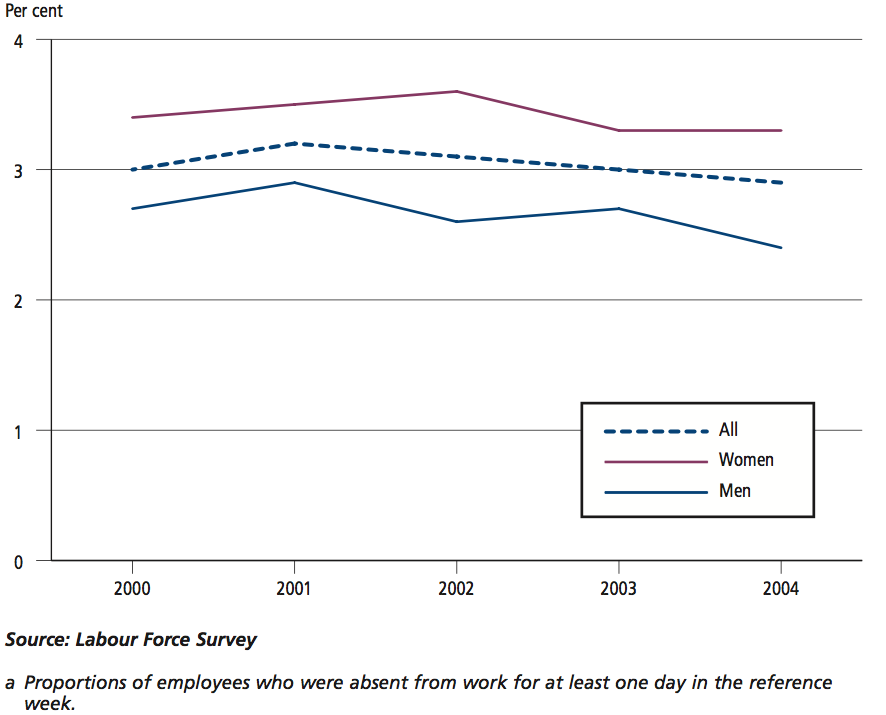
\includegraphics[width=0.5\textwidth]{images/men_women_sick.png}}
        \item<4->[Age]: Junior staff (16-34) are most likely to be absent
        \only<4>{ 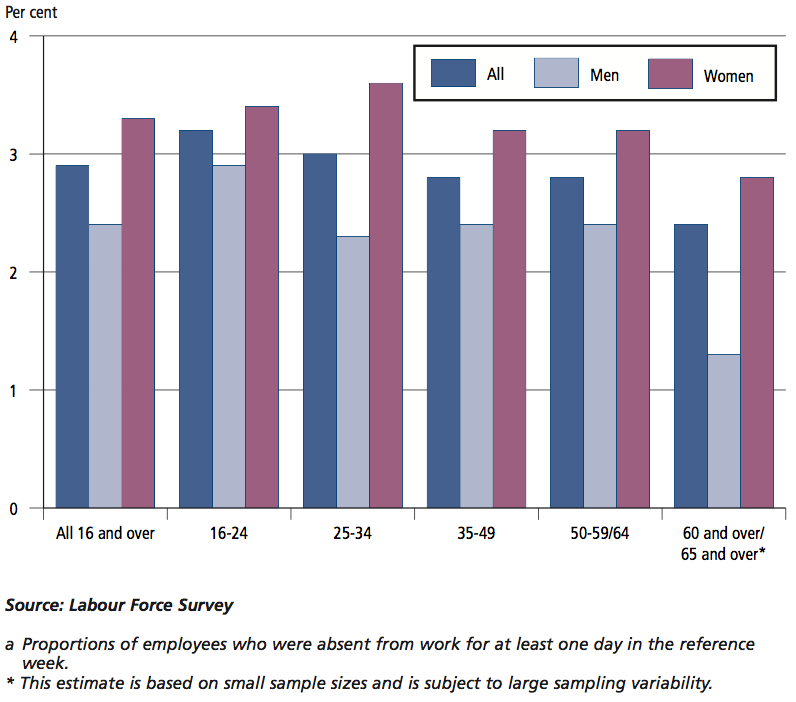
\includegraphics[width=0.5\textwidth]{images/young_old.png}}
        \item<5->[Weekday]: Midweek absences are most likely
        \only<5> {
        \medskip
        \tiny
        \begin{tabular}{| l | c | c | c | c | c | c | c | }
  \hline			
  Day:      & Mon    & Tue    & Wed    & Thu    & Fri    & Sat   & Sun \\ \hline
  Absences: & 17,670 & 19,051 & 19,115 & 18,914 & 17,883 & 4,610 & 2,520 \\
  Percent: & 17.7 & 19.3 & 19.0 & 19.1 & 18.5 & 4.1 & 2.3 \\
  \hline  
\end{tabular}
        }
    \item<6->[Profession]: Industry, role and Public/Private are predictive
    \item<6->[Location]: Londoners are more likely to be sick (3.1\%) compared to non-Londoners (2.2\%)
    \item<7->[Recurrence]: Frequent absentees have a higher risk of future absences, and long-term absences
    \item<8->[Season]: Absences peak in Winter months, and are minimal in Summer months
    \end{description}
}
    
\end{frame}


\begin{frame}{Sick-Leave Patterns \& Indicators}

Final Feature Set
\begin{itemize}
    \item Gender (via name) : Categorical (3)
    \item Project role (proxy for age) : Categorical (?)
    \item Weekday : Categorical (7)
    \item Individuals' sick-leave days in the last  12 months : Numeric
    \item Teams' sick-leave days in the last four weeks : Numeric
    \item Time of Year: encoded using a number of Fourier terms ? $\times$ numeric
    \begin{itemize}
        \item For day $d$ produce a 2-vector $\left(cos(2\pi \frac{d}{365}), sin(2\pi \frac{d}{365})\right)$.
    \end{itemize}
\end{itemize}
\medskip
Ignore
\begin{itemize}
\item Location
\end{itemize}


\end{frame}


%--- Model ----------------------------------%

\section{Model}
\begin{frame}{Baseline Model}

Baseline Model
\begin{itemize}
    \item Average per-month absenteeism by gender 
\end{itemize}

\only<2-> {
    Prediction:
    
    \begin{itemize}
        \item For a given month $m$
        \item When individual $u$'s absentee rate is $a_{um}$ 
        \item In which a 15-day sprint occurs   
        \only<3> {
        \item $\Pr(\text{absences} = y | \text{sprint} = s, \text{month}=m, \text{user}=u) = \text{Bin}\left(a_{um}, 15 \right)$
        }
        \only<4> {
        \item Expected number of absences for an individual $u$ is $15 a_{um}$
        }
        \only<5> {
        \item The expected number of absences in a team is $T . 15 \left(\frac{1}{T}\sum_{u \in T} a_{um}\right)$ 
        \item The variance is $T \bar{a}_m \left(1 - \bar{a}_m\right) - \sum_{u \in T}\left(a_{um} - \bar{a}_m\right)$ (see \cite{DreznerFarnum1993})
        }
    \end{itemize}
}

\end{frame}

\begin{frame}{Custom Model}
Logistic Regression; L2-Regularization via Spherical Gaussian prior
\medskip
Denote the variable extracted from a record as $\phi(x)$
\begin{align*}
p(y|x) & = \sigma(\mathbf{w}^\top \phi(x)) \\
\mathbf{w} & \sim \mathcal{N}\left(\mathbf{0}, \tau^{-1} I\right)\\
\tau &\sim \mathcal{G}\left(a_0, b_0\right)
\end{align*}

Use Probit trick\cite{Bishop2006} for prediction
\begin{align*}
p(y^*|x^*y,X) & = \int \sigma(\mathbf{w}^\top \phi(x^*)) p(\mathbf{w} | y, X) d \mathbf{w} \\
& \approx \sigma(\kappa(\phi(x^*)\Sigma^{(w)}_{N}\phi(x^*)) \quad \mathbf{w}_{\text{MAP}}^\top \phi(x^*))\\
\kappa(\alpha^2) & = (1 + \pi \alpha^2 / 8)^{1/2}
\end{align*}

\end{frame}

\begin{frame}{Custom Model : Expediting Training 1}

\begin{itemize}
\item<1-> Inference in Bayesian logistic classically involves a second-order Taylor expansion around the posterior mode to handle the model's non-conjugacy: the Laplace approximation
\item<2-> This involves evaluating and inverting the Hessian at every iteration
\item<3-> The Bohning bound\cite{BohningLogReg1988} replaces the true Hessian with an upper bound: $\hat{\text{H}} = \frac{1}{2}\left(I - \frac{1}{2}\mathbf{1}\mathbf{1}^\top\right)$, $\quad\hat{\text{H}}^{-1} = 2\left(I + \mathbf{1}\mathbf{1}^\top\right)$
\item<4-> This reduces the time per iteration, and guarantees convergence, but increases the number of iterations involved
\end{itemize}
\end{frame}

\begin{frame}{Custom Model : Expediting Training 2}

The dataset is heavily skewed, so focus only on positive examples and skip negative ones, using weighted stochastic gradient descent\cite{Gopalan2013b}[supporting material]\\
\medskip
\only<1> {
SGD
\begin{align*}
\mathbb{E}_{p^*}[D \cdot f(x)] & \approx \frac{D}{S}\sum_s f(x_s),\quad &
x_s & \sim p^* \qquad p^*(x) = \frac{1}{D} \sum_d 1_{x = x_d}
\end{align*}\begin{align*}
& & \mathbf{w} & \leftarrow \mathbf{w} - \eta \nabla_{\mathbf{w}} \frac{D}{S}\sum_s f(x_s)
\end{align*}
}
\only<2,3> {
Weighted SGD \\
Use a proposal distribution $q(x)$ selecting negative examples with small probability $\epsilon$ and positive examples probability $1-\epsilon$
}\only<2> {
\begin{align*}
\mathbb{E}_{p^*}[D \cdot f(x)] & = \mathbb{E}_{p^*}[D \cdot f(x) \frac{q(x)}{q(x)}] \\
& \approx \frac{D}{S}\sum_s f(x_s) \frac{p^*(x_s)}{q(x_s)} q(x_s) \\
& \approx \mathbb{E}_{q^*}[D \cdot f(x) \frac{p^*(x)}{q(x)}]
\end{align*}
}
\only<3> {
\begin{align*}
\mathbf{w} & \leftarrow \mathbf{w} - \eta \nabla_{\mathbf{w}} \left(\frac{D^-}{S \epsilon}\sum_s f(x^-_s) + \frac{D^+}{S (1 -\epsilon)}\sum_s f(x^+_s)\right)
\end{align*}
}

\end{frame}

\begin{frame}{Custom Model : Open Questions}

\begin{enumerate}
    \item Do Sharktower customers' behaviours match the Labour-Force Survey
    \item Are there any interactions between features
    \item How many Fourier terms are needed to model seasonality
    \item Does the Bohning bound interact poorly with SGD. If so consider the local Jaakola bound\cite{Jaakkola1997} instead.
\end{enumerate}

\end{frame}


%--- Evaluation ----------------------------------%

\section{Evaluation}
\begin{frame}{Evaluation}

\begin{itemize}
    \item Incidence is too low for simple accuracy, so use ranking metrics
    \item Ranking metrics include
    \begin{itemize}
        \item Precision at M: what proportion of the top M ranked employees were in fact absent
        \item Recall at M: what proportion of all absent employees (clamped at M) were in the top M
    \end{itemize}
        
    \item Can also compare actual team absences per month with expected team absences
\end{itemize}

\end{frame}

%--- Engineering ----------------------------------%

\section{Engineering}
\begin{frame}{Engineering}

Resources
\begin{description}
    \item[Tools]: Python stack: Numpy, Scipy, Scikit-Learn
    \item[Data (Internal)]: Full list of absences for all members of all teams of all clients with forenames, team IDs and project roles
    \item[Data (External)]: A name to gender database: likely to start with: {\small http://www.cs.cmu.edu/afs/cs/project/ai-repository/ai/areas/nlp/corpora/names/ }
\end{description}
Sprint Work:
\begin{description}
    \item[Week 1]: Acquiring and cleaning data, feature-extraction, train-set \& validation set, name-to-gender model
    \item[Week 2]: Baseline model, PoC of custom model, evaluation on validation.
    \item[Week 3]: Refinements of baseline model, discussion with engineering for productionization if suitable.
\end{description}



\end{frame}

%--- Engineering ----------------------------------%

\section{Questions}
\begin{frame}{Questions}

Questions



\end{frame}



%--- the Bibliography frame -------------------------%

\section{References}
\begin{frame}[allowframebreaks]{References}

{\tiny 
    \bibliographystyle{plain}
    \bibliography{/Users/bryanfeeney/Documents/library.bib}
}

\end{frame}



\end{document}
